\documentclass[10pt,a4paper]{article}
\usepackage[latin1]{inputenc}
\usepackage{amsmath}
\usepackage{amsfonts}
\usepackage{amssymb}
\usepackage{float}
\usepackage{listings}
\usepackage{graphicx}
\usepackage[usenames,dvipsnames]{color}

\begin{document}
\definecolor{light-gray}{gray}{0.90}
\lstset{language=Python,breaklines=true,backgroundcolor=\color{white},frame=single}

\author{Jeroen Hofman\\
		10194754\\
		}
\title{Computer exercises week 39, 2011\\
		}
\date{}
\maketitle

\subsection*{Exercise 5.18}
Code:a
\begin{lstlisting}
#the vector g
def g(x,y):
    gx = (x+3)*(y*y-7)+18
    gy = sin(y*exp(x)-1)
    return np.array([gx,gy])

#the Jacobian
def Jac(x,y):
    j1 = y**3 - 7
    j2 = 3*(x+3)*y*y
    j3 = exp(x)*y*cos(exp(x)*y-1)
    j4 = exp(x)*cos(exp(x)*y-1)
    return np.matrix([[j1,j2],[j3,j4]])

x0,y0 = -0.5,1.4
n = 20

#Newton's method
for k in range(0,n):
    print x0,y0
    print "k = ",k," error = ",x0+y0-1
    s = solve(Jac(x0,y0),-g(x0,y0))
    x0 += s[0]
    y0 += s[1]

x0,y0 = -0.5,1.4
Jaco = Jac(x0,y0) 
n = 100

#Boydens method
for k in range(0,n):
    print x0,y0
    print "k = ",k," error = ",x0+y0-1
    s = np.transpose(solve(Jaco,-g(x0,y0)))
    x0 += s[0]
    y0 += s[1]
    z = g(x0,y0)-g(x0-s[0],y0-s[1])
    Jaco = Jaco + (np.outer((z - np.dot(Jaco,s)),s))/(np.dot(s,s))
\end{lstlisting}

\noindent In this exercise we solve a system of nonlinear equations. In the two function definitions above we have computed the solution vector and the Jacobian respectively. We now use Newton iteration first with a starting vector of $x = \{-0.5,1.4\}^{T}$ to obtain the solution for the system. By computing the infinity norm of the error the Newton iteration attains full machine precision after 15 steps. We can do the same procedure for Boydens method, calculating the infinity norm of the error in each step as we go through the algorithm. Boydens method reaches full machine precision after 11 steps, hence it is a little faster than Newtons method.

\subsection*{Exercise 6.7}

\noindent In this exercise we study the behaviour of the function $f(x,y) = 2x^3 - 3x^2 -6xy(x-y-1)$. The critical points of this function are already analysed in exercise 6.5c, and from that exercise we obtain 2 saddle points, (0,0) and (0,-1), a local maximum (-1,-1) and a local minimum (1,0). Below a contourplot is given for the function for $-2 < x,y < 2$. We used a numerical minimizer routine in Mathematica (NMinimize) to verify the minimum we found at (1,0). The dots seen in the figure are the iterations of the minimizer routine. Using this method we can also investigate the maximum by using NMinimize on -f, producing a similar picture as below, and this method indeed gives the local maximum (-1,-1).\\
\begin{center}
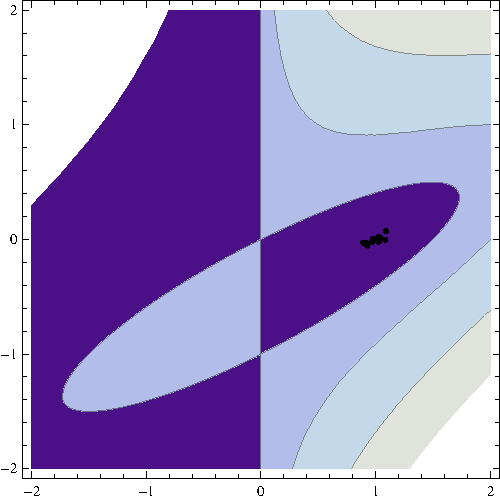
\includegraphics{plot.pdf}
 \end{center}
 
\subsection*{Exercise 6.7b}
Code:
\begin{lstlisting}
f = open('/home/jhofman/Desktop/NA/NA week 40/path3.txt','w')

def gradg(x,y):
    gx = 200*(y-x*x)*-2*x -2*(1-x)
    gy = 200*(y-x*x)
    return np.array([gx,gy])

def Hes(x,y):
    j1 = 1200*x*x-400*y+2
    j2 = -400*x
    j3 = -400*x
    j4 = 200
    return np.matrix([[j1,j2],[j3,j4]])

x0,y0 = 2.0,1.0
n = 10
for k in range(0,n):
    print x0,y0
    f.write(str(x0)+' '+str(y0)+'\n')
    s = solve(Hes(x0,y0),-gradg(x0,y0))
    x0 += s[0]
    y0 += s[1]
\end{lstlisting}

\noindent In this exercise we use Newtons method for more dimensions to minimize the function $f(x,y) = 100(y-x^2)^2 + (1-x)^2$. We calculate the Hessian matrix and the Jacobian of this function given above, defined in Hes(x,y) and gradg(x,y) respectively. We then solve this system by Newton iterations, i.e. solving $H(x0,y0) s_{0} = - \triangledown f(x0)$ with some inital guess $(x0,y0)$. I have used $(-1,1),(0,1)$ and $(2,1)$ as starting points. The figure below shows the successive iterations of the solution to the exact solution $(1,1)$. In all three cases within 5 iterations the exact solution is reached within machine precision, hence this method is very fast.\\
\begin{center}
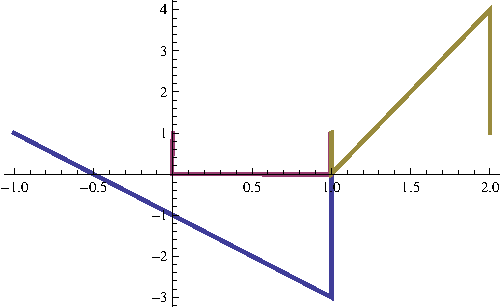
\includegraphics{plot2.pdf}
\end{center}
\end{document}